\documentclass{sig-alternate}
\usepackage{color}
\usepackage[colorinlistoftodos]{todonotes}
\usepackage{amssymb}
\usepackage{upgreek}
\begin{document}
\conferenceinfo{UMM CSci Senior Seminar Conference, December 2014}{Morris, MN}

\title{Gait Recognition in Mobile Security}

\numberofauthors{1}

\author{
\alignauthor
Chase R. Ottomoeller\\
	\affaddr{Division of Science and Mathematics}\\
	\affaddr{University of Minnesota, Morris}\\
	\affaddr{Morris, Minnesota, USA 56267}\\
	\email{ottom005@morris.umn.edu}
}

\maketitle




\begin{abstract}
This paper discusses a new form of mobile security, emphasizing both security and convenience. Having a form of security on a mobile device that is unobtrusive can make that device easier to use. Using built-in accelerometers in smart phones as a way to collect biometric data is one of these forms. In this case the biometric data is a person's gait, or walking pattern. This increases the security of the device by allowing the authentication to be something you are rather than something you have or something you know. There are two example that this paper will compare, showing two forms of gait analysis. Though both studies are a work in progress, they both implement working security schemes, allowing the phone to  verify the user's identity correctly.  
\end{abstract}

\keywords{mobile authentication, gait recognition, biometrics, accelerometer,linear interpolation, dynamic time warping}



%1111111111111111111111111111111111111111111111111111111111111111111111111
\section{Introduction}
	Computational power in computers continues to increase as technology advances. Security is a growing concern, particularly regarding security of mobile devices such as smart phones. The current methods to unlock smart phones will soon be vulnerable to brute force  attack, which is an attack that tries all possible combinations of a password. Common security authentication methods include: pin, password, swipe lock, token, and fingerprint. Most of these methods are either something a person has (card, token, key) or something a person knows (password). They all require a physical action to unlock the phone. A new form of mobile security involves biometrics. Using biometrics allows the device to identify a person based on their characteristics (fingerprint) and not by what they have or what they know.  One form of biometrics being explored uses a person's gait or walking pattern. 
	%This  making it an unobtrusive form of security.
	
	This paper analyzes two different approaches for gait recognition and analysis. Each approach uses a general process to extract and analyze the data which includes: Preprocessing, Feature Extraction, and Gait Analysis. \textit{Preprocessing} is the process of taking the raw accelerometer data and preparing it for feature extraction. \textit{Feature Extraction} is taking the preprocessed biometric data, and locating distinctive characteristics within that data. \textit{Gait Analysis} is taking the features extracted from the data, and comparing them against a predefined template. This comparison determines if the current user is an imposter or not.

	In the following sections, I will be comparing two approaches of gait recognition using accelerometers from a mobile device, such as a smart phone. These two approaches use different placement of the mobile device on the body. This difference in placement impacts the techniques that are used to recognize and analyze gait patterns. One approach has the smart phone in a fixed location on the waist. I will refer to this method as the \textit{fixed} method. The other method has the smart phone in a more natural position on the body such as in a pocket. This method will be referred to as the \textit{unfixed} method. Though both methods use a complex approach shown in figure~\ref{fig:AlgorithmProcess}, I will simplify comparisons between these methods. I will group them into three categories: Preprocessing, Feature Extraction, and Gait Analysis. 
	
%1111111111@@@@@@@@@@@@@@@@@@@@@@@@@@@@@@@@@@@@@@@@@@@@@@@@%
\begin{figure}
\centering
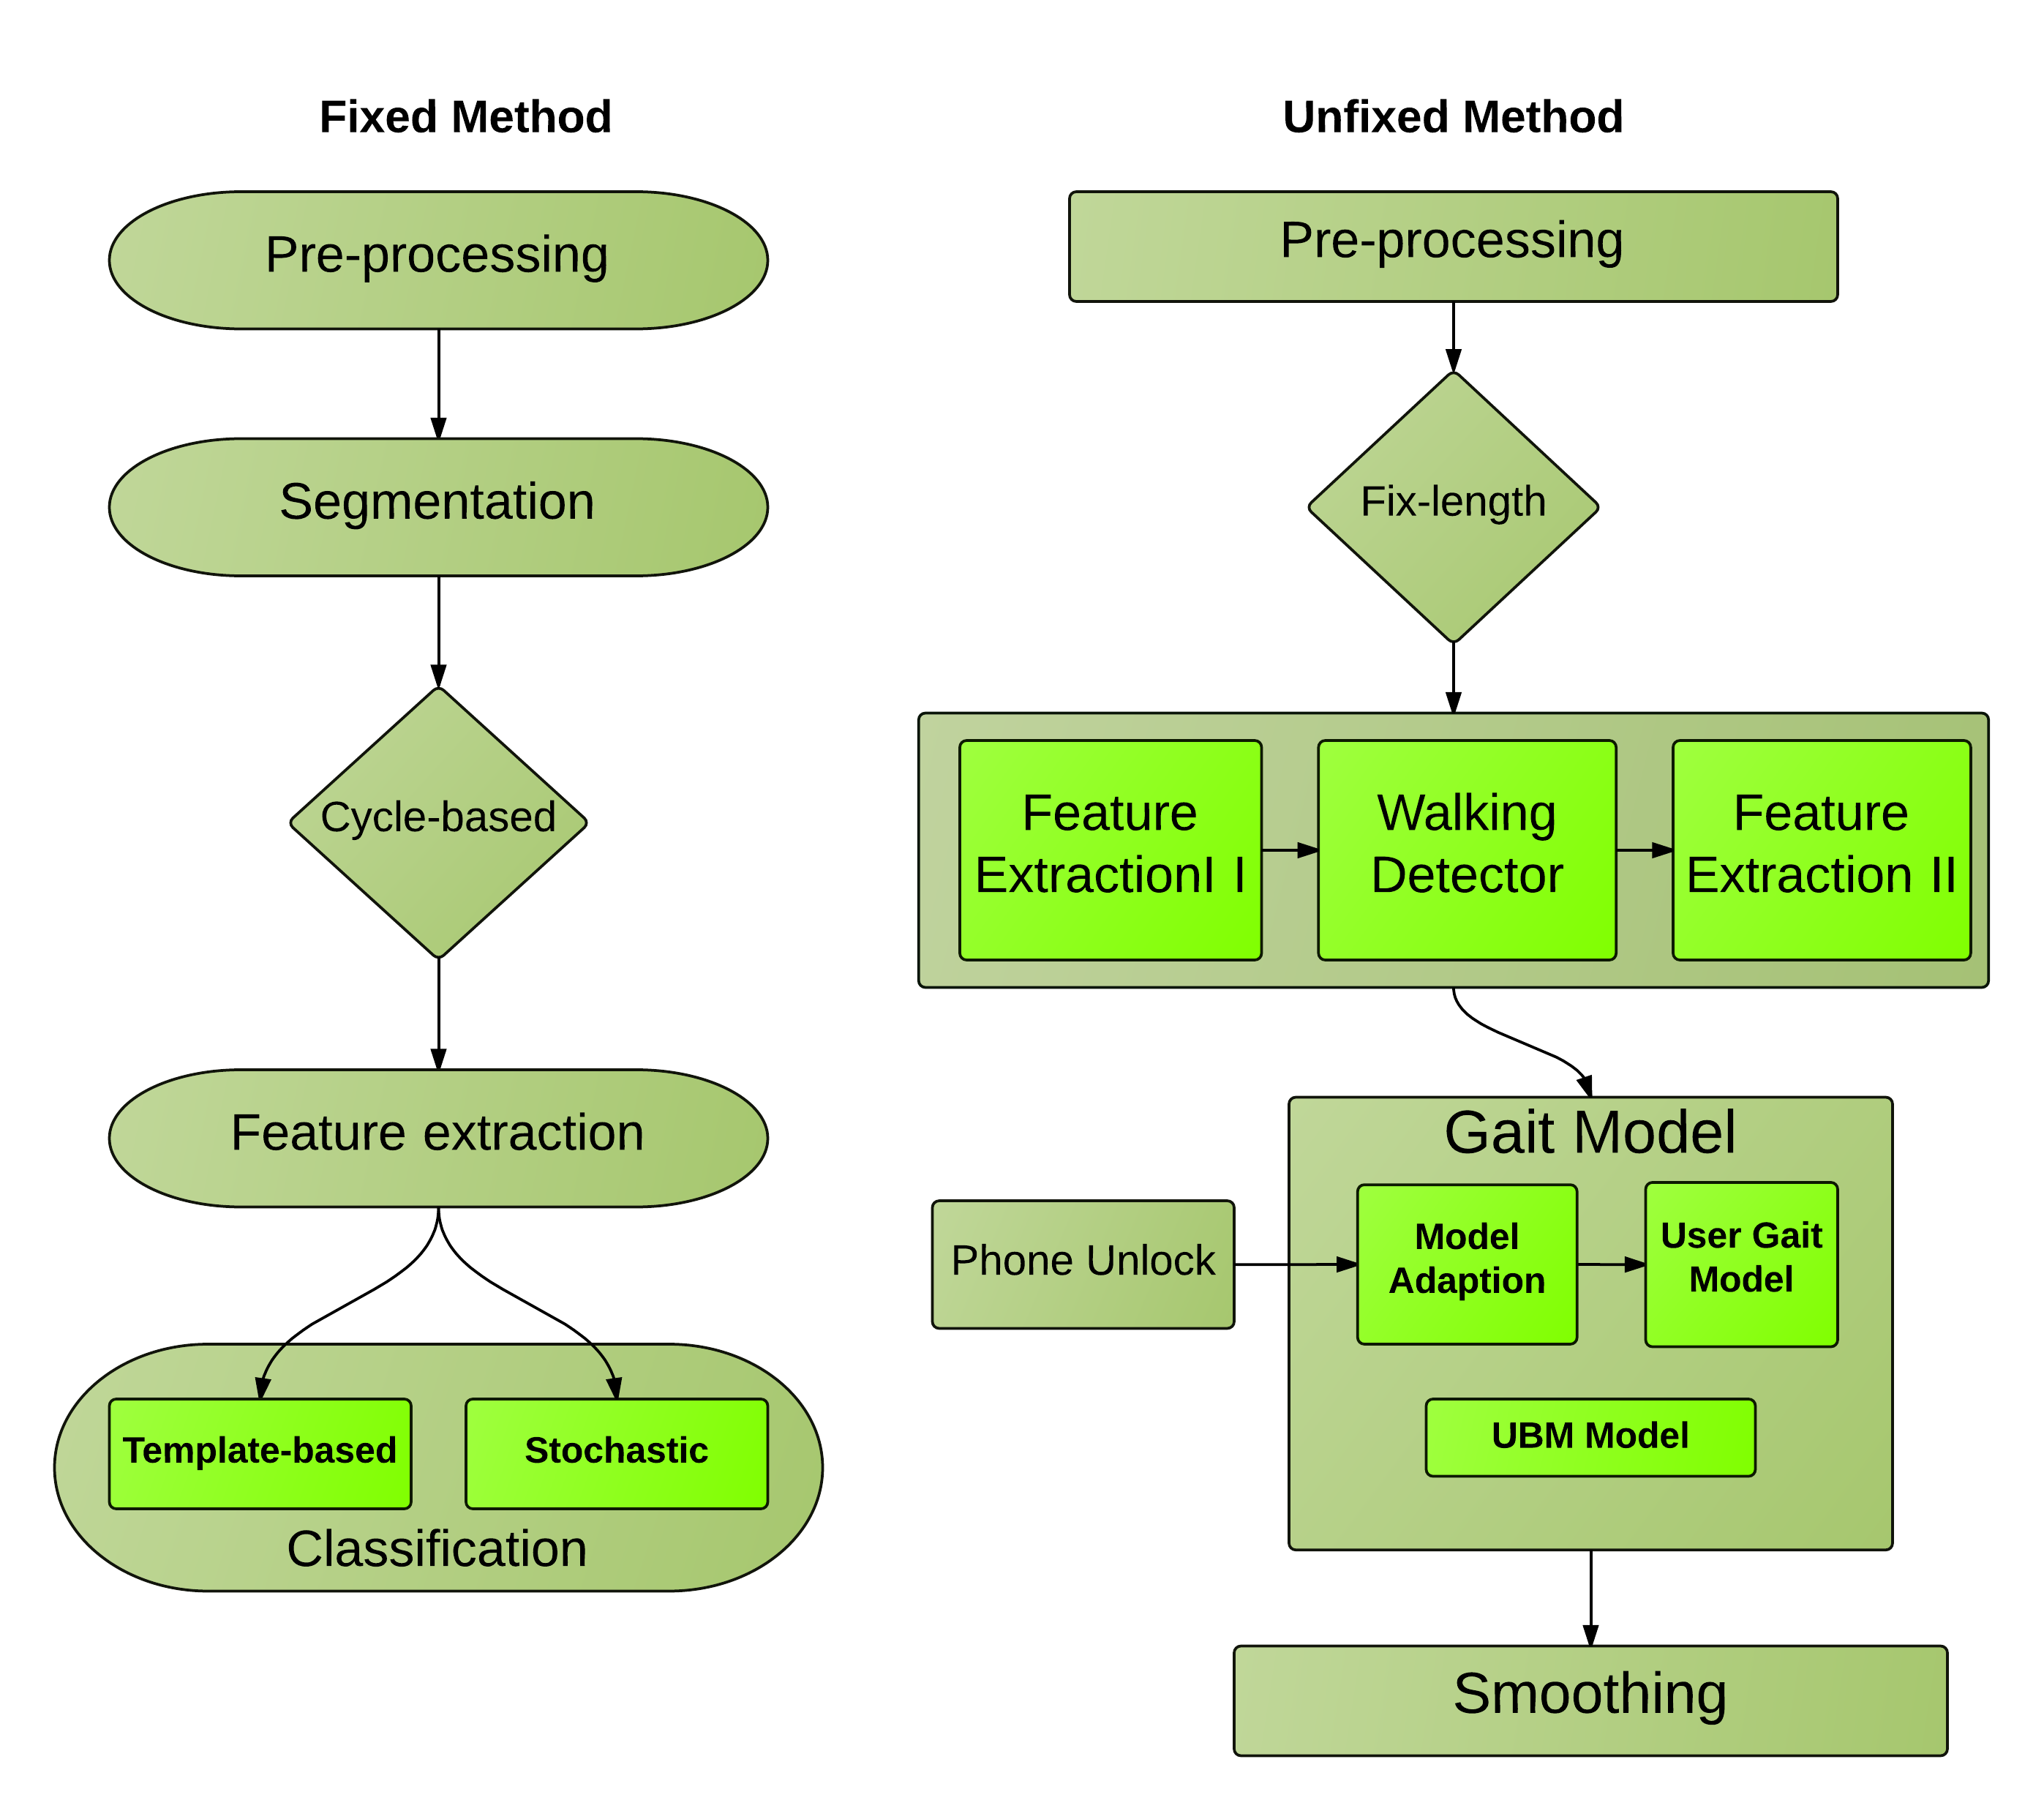
\psfig{file=AlgorithmProcess.png,height =3.2in, width =3.5in}
\caption{Different Approaches to Gait Recognition}
\label{fig:AlgorithmProcess}
\end{figure}	
%@@@@@@@@@@@@@@@@@@@@@@@@@@@@@@@@@@@@@@@@@@@@@@@@%%

%I plan to use the following sources:
%\begin{itemize}
%\item one~\cite{Sujithra:2012}
%\item two~\cite{Muaaz:2013}
%\item three~\cite{Lu:2014}
%\end{itemize}


%222222222222222222222222222222222222222222222222222222222222222222222222222222
\section{Background}
	Biometrics can be used as a new form of security by identifying characteristics that are unique to the mobile user. Instead of relying on a password or physical key, a person can gain access to their device by a physical characteristic specific to them. Biometrics can be split into two categories, physiological and behavioural. Physiological biometrics include: Finger Scan, Facial Scan, Iris Scan, and DNA Matching. Behavioural biometrics include: Voice Recognition, Keystroke Scan, and Gait Recognition. In this paper, I will focus on gait recognition. The term gait refers to the walking pattern of a person. A person's walking pattern is cyclic in nature and may be composed of many gait cycles, where each gait cycle consists of at least two steps.~\cite{Sujithra:2012} 
	
	In mobile security, when gait recognition is used, gait data is collected via the built-in accelerometer of the smart phone. The smart phone will use the collected data to analyze a person's walking pattern. If the phone can determine that the current user should have access, the phone will be unlocked. If the gait is not recognized, the phone will switch to a different authentication method such as pin access. This method increases the security of the mobile device, because the form of unlocking the device is now a personal characteristic (a biometric) and something that is not likely stolen, forgotten, or forged. Other biometrics, such as a fingerprint that can be copied, an imposter would have trouble replicating a gait pattern.



%333333333333333333333333333333333333333333333333333333333333333333333333333333333333333
\section{Two Research Cases: Fixed \\ Method and Unfixed Method}
	The research group that employed the fixed method did two experiment set-ups: Template-based classification and Machine learning based classification. The data set was made from 51 subjects (39 males, 12 females) that walked down a 18.5 meter long corridor. The template approach selects the best cycle from the data set and compares it to a ``template" that represents the correct user's gait. If the selected cycle doesn't match the template, then authentication has failed, and the phone is locked.  The fixed method also uses Support Vector Machines(SVM's) for the machine learning approach. The basic idea of SVM's is taking dimensional data and separating it into two classes. This involves the use of a gaussian kernel defined in the following section. The accuracy of this method is measured by the Equal Error Rate (EER). This is the rate at which both the acceptance and rejection errors are equal
	
	The unfixed method experimented using 3 data sets all using Android phones. The first data set included 49 people, 19 female and 28 male. These subjects performed various tasks that included: standing, sitting, walking, biking, running, driving, and random movements. The second data set was made up of 12 people, 5 female and 7 male. These subjects did tests in a more controlled environment with different phone placements, walking distances, and walking speeds. The third data set was designed to collect data in a real-life setting. This involved 8 people that collected data for 5 hours each. This method uses a Gaussian Mixture Model - Universal Background Model (GMM-UBM) framework to verify an individual's gait. To verify an individual's gait, a technique involving scoring is used. Verification of a user's identity is done by comparing the likelihood score from a user's gait pattern to the universal background model. The universal background model represents human gait patterns in general. 


\section{Preprocessing} 
	Once data is gathered, it needs to be preprocessed into a usable form. This is done by separating the data into pieces. In the following sections, I will explain the fixed and unfixed methods of preprocessing.

    
\subsection{Fixed Method Preprocessing}	\label{FPP}
	With the phone on the waist in a fixed position, uniform sets of data, called \textit{walks}, were collected. One walk is defined by walking a measured distance down a hallway. The experiment was conducted so that one set of data contained two ``walks''. In other words, one set of data was walking down a hallway, once down and once back. After being extracted, the raw gait data is preprocessed using two steps: \textit{linear interpolation} and \textit{zero normalization}. 
			
\subsubsection{Linear Interpolation} \label{LI}
	Since the built-in accelerometer does not output data in equal intervals, the data needs to be reshaped into equal intervals. This is done by applying \textit{linear interpolation}. To avoid losing data during this change, up-sampling can be applied. Up-sampling avoids data loss by producing ``an approximation of the sequence that would have been obtained by sampling the signal at a higher rate''~\cite{wiki1:2014}. Once the data has been reshaped, the acceleration measurements have to be adjusted to account for unstable accelerometer readings. 
			
\subsubsection{Zero Normalization}
	The mobile device's accelerometer is used to measures 3 axes (X, Y, Z). The only axis needed, and the only axis affected by gravity is the X axis. Since the acceleration for the Y and Z axes are not stable over time and they are not affected by earth's gravity, the acceleration data for the Y and Z axis have to be \textit{zero normalized}. In other words, the data for the Y and Z axes have to be set to zero. This is done by simply subtracting their total acceleration from their average acceleration. An overview of the stages explained above are shown in figure ~\ref{fig:firstStep}.
	
%2222222222222222@@@@@@@@@@@@@@@@@@@@@@@@@@@@@@@@@@@@@@@@@@@@@@@@%
\begin{figure}
\centering
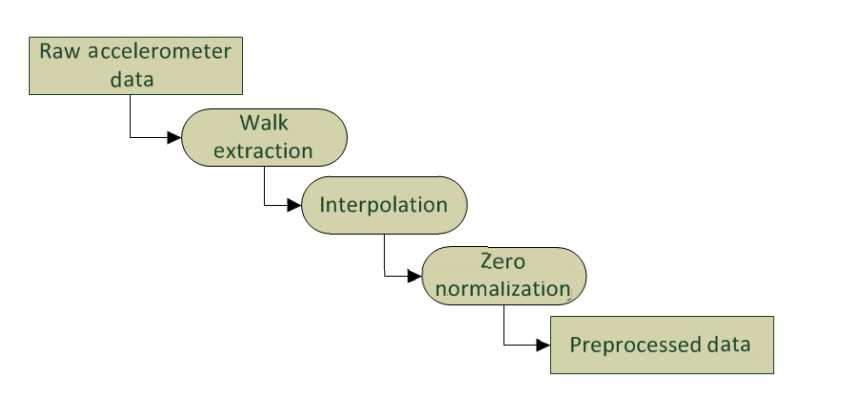
\psfig{file=chart1.png,width =3in}
\caption{Fixed Method Preprocessing Step}
\label{fig:firstStep}
\end{figure}

%@@@@@@@@@@@@@@@@@@@@@@@@@@@@@@@@@@@@@@@@@@@@@@@@%
	
\subsection{Un-fixed Method Preprocessing}{
	The previous method used a phone in a fixed location. This method expands from having the phone on the waist, to having the phone in a unfixed location, such as a pocket. Also, this method does not use a set length, such as a hallway, making it more flexible. This method marks each walk using a method called called \textit{framing}. Framing separates the data into sets of equal time. Once the data is segmented into frames, it is then projected onto a global coordinate system through a process know as \textit{projection}.}
		
		
			
\subsubsection{Framing}{
 During Framing, sensor data is segmented into uniform frames for feature extraction and feature classification. This is similar to the preprocessing of the data for the fixed method. The fixed method had its data separated into ``walks''. This data, not having the separation of ``walks'', is separated into sections of 512 equal samples in length. This is done by separating sections every 5.12 seconds. The reason for 512 samples was ``to balance between estimation accuracy and latency.''~\cite{Lu:2014} This was to maintain balance between the accuracy of matching a user and the time it took to compute the match. Not all frames move onto feature extraction. Frames that are below a chosen threshold, representing no movement, are dropped. }
 			
\subsubsection{Projection}{
	Each sample within a given frame contains an X, Y, and Z coordinate. Each coordinate is then projected into a vertical and horizontal variable. Once each sample is projected, the direction of gravity is determined by using a mean filter. Unlike the previous example, this process does not assume a fixed location or orientation of the mobile device. In order for the device to record accurate data from the accelerometer, the devices orientation (up, down, left, and right) must be accurate. If there is a significant change in the gravity variable then the orientation of the device has changed. This means the corresponding frame will be dropped and the horizontal and vertical axes will be adjusted accordingly. 
}
\subsection{Comparison of Preprocessing Approaches}
	Both the fixed and unfixed methods split the data into equal intervals as well as modify the data so that it is in a useful form. The reason for the differences between the preprocessing methods stems from the differences in phone placement. The data collected in the fixed method is already more organized than the data from the unfixed method. This is because the unfixed method has to account for multiple axes as well as data unrelated to gait. If the fixed method were to be implemented in more of a realistic scenario then these methods become even more similar. 

%444444444444444444444444444444444444444444444444444444444444444444444444444
\section{Feature Extraction}
	\textit{Feature Extraction} is extracting a set of data from a given frame to detect patterns of walking. Another way to define feature extraction is the process of extracting gait cycles from the data. 		
\subsection{Fixed Method Feature Extraction}\label{FFE}
	To extract gait cycles from the preprocessed data, the fixed method uses the following steps in order, as seen in Figure~\ref{fig:SecondStep}: Cycle length estimation, Cycle detection, Cycle length normalization, and Omitting unusual cycles. 
	
%333333333333333@@@@@@@@@@@@@@@@@@@@@@@@@@@@@@@@@@@@@@@@@@@@@@@@%
\begin{figure}
\centering
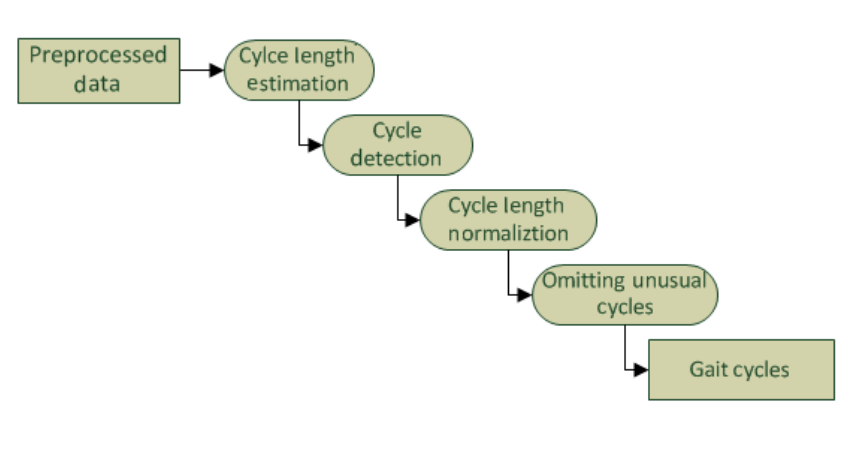
\psfig{file=chart2.png,width =3in}
\caption{Fixed Method Feature Extraction Step}
\label{fig:SecondStep}
\end{figure}

%@@@@@@@@@@@@@@@@@@@@@@@@@@@@@@@@@@@@@@@@@@@@@@@@%
			
\subsubsection{Cycle Length Estimation}
	Once the raw gait data is preprocessed, the next step is extracting the gait cycles. The first step in extraction is to automatically detect gait cycles in the walk. This detection is done by estimating the cycle length, done by computing the \textit{salience vectors}. In this scenario, a salience vector is the distance measurement from one chosen data point of a cycle to another chosen data point. A minimum and maximum salience vector is computed for each data point for a given walk. Each minimum salience vector is computed by counting the data values that are between the current data value and the following smaller value in the walk vector. The same process is used for maximum salience vectors, but instead of calculating the distance to the next smallest value, it is calculating the distance to the next largest value. The number of values counted is the distance measurement for that data point. The minimum salience vectors with the greatest distance measurements are considered cycle starts. Sometimes there is more than one minimum salience vector, making the start of a cycle unclear. Maximum salience vectors help to verify the start of cycles because they occur right after the cycle start.
			
\subsubsection{Cycle Detection}
	Once both minimum and maximum salience vectors are computed, they can be used to detect individual cycles. Figure~\ref{fig:AccelChart} shows a set of accelerometer data, and the corresponding salience vector distance measurements. The start of each cycle is based on the minimum salience vector. There are spikes at time points 750, 1150, 1450, and 1650. These spikes indicate where a distance measurement for a data point is larger than the rest. These spikes are the minima calculated from the minimum salient vector. These minima mark the start of gait cycles. If there is a cycle that is longer than the rest, the minimum and maximum salient vectors are computed again. This will split the cycle into smaller ones, giving more uniformity to the data. Uniformity of the data is needed for the next step of normalizing the data.

%4444444444@@@@@@@@@@@@@@@@@@@@@@@@@@@@@@@@@@@@@@@@@@@@@@@@%
\begin{figure*}
\centering
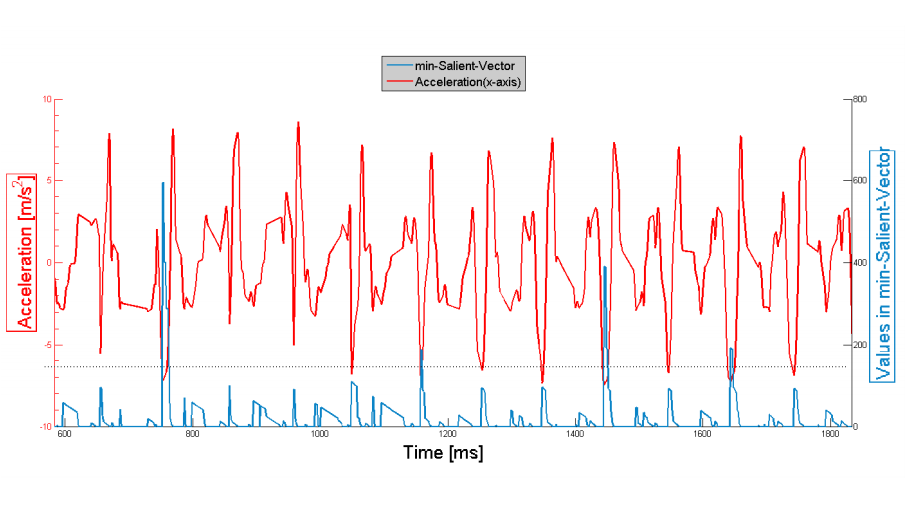
\psfig{file=svector.png,height =2.5in,width =5.3in}
\caption{Minimum Salient Vectors}
\label{fig:AccelChart}
\end{figure*}

%@@@@@@@@@@@@@@@@@@@@@@@@@@@@@@@@@@@@@@@@@@@@@@@@%
			
\subsubsection{Cycle Length Normalization}
Once the start of each cycle is determined, the cycle distance is measured from the start of once to the start of the following cycle. Different cycles may have different lengths. As described in \ref{LI}, by using linear interpolation the determined cycles are normalized to a set length. Equal cycle lengths are required for some of the feature extraction techniques. 
			
\subsubsection{Omitting Unusual Cycles}
Some cycles, in comparison with the majority, are considered unusual. These could be caused by any motion or non-motion that does not correspond to walking. Such patterns are detected by ``computing the distance using \textit{Dynamic Time Warping} (DTW).''~\cite{Muaaz:2013} DTW is ``an algorithm for measuring similarity between two temporal sequences which may vary in time or speed.''~\cite{wiki2:2014} This means that cycles with an acceleration of half or less of the other cycles will be removed. Since this method positions the phone on the waist, and the data was collected in a controlled environment, there will be fewer unusual cycles removed in the fixed method than in the unfixed method. This is further explained in the following section.

\subsection{Unfixed Method Feature Extraction}
	A different form of extraction used by~\cite{Lu:2014} is separated into three stages: Feature Extraction I, Walking Detection, and Feature Extraction II. Feature Extraction I is used to get rid of any unwanted and incorrect data, such as data collected when the phone changes position. Walking Detection is used to specify what kind of motion the current data set represents, such as biking, running, or walking. Feature Extraction II pulls the gait data from the data set to be analyzed. 
%5555555555555555555555555@@@@@@@@@@@@@@@@@@@@@@@@@@@@@@@@@@@@@@@@@@@@@@@@%
%\begin{figure}
%\centering
%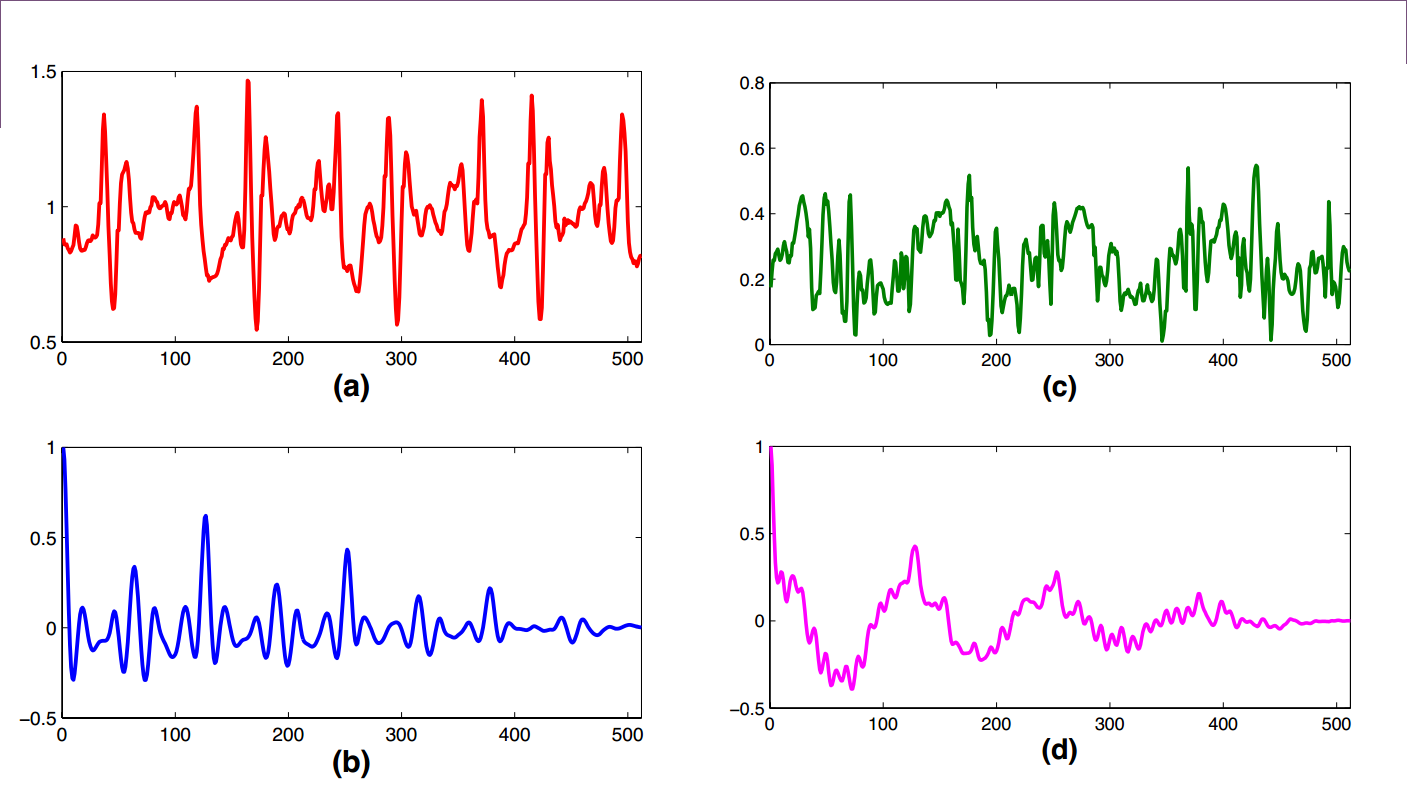
\psfig{file=abcd.png,width =3in}
%\caption{(a) and (b) represent horizontal and vertical components recorded by the accelerometer. (c) and (d) represent the horizontal and vertical components after the data has been normalized.}
%\label{fig:TD1}
%\end{figure}
%@@@@@@@@@@@@@@@@@@@@@@@@@@@@@@@@@@@@@@@@@@@@@@@@%	


\subsubsection{Feature Extraction I}
	 Unlike the fixed method with the very specific context for what is and isn't walking, the unfixed method has data representing multiple types of motion. Motion such as riding a bike, or riding in a vehicle. For example, if the mobile device was collecting data when it was in a car going down the road, that data should not be used to extract features. This is because this data is not gait data. This also holds true for collecting data on someone who is standing still. The data collected would not represent the data needed for gait recognition.
	 
% 	The first stage of the feature extraction is used to tell whether the data represents walking or if the data represents some other activity. Differentiating between walking and non-walking helps further classify the data in \ref{WD}.%
 	
	To determine the type of motion, such someone walking, both time domain and frequency domain are used. For example, a time domain graph would show how a signal changes over time. A frequency domain graph would show how much of a signal lies within a given frequency band. The frequency domain uses spectrum analysis to estimate the strength of different frequency components of a time domain signal. In other words, performing ``different activities have different energy distributions over the frequency spectrum.''~\cite{Lu:2014} Walking can be measured around 1-2Hz while performing other activities, such as driving in a car, will output a higher frequency band (>3Hz). These features are used for walking detection in the following step.
			
\subsubsection{Walking Detection} \label{WD}
	Using the features calculated from Feature Extraction I, classification can be performed using a decision tree. There are three activities that the data can be classified as: walking, non-walking, and random movements. Walking motion (1-2Hz) is defined as motion created by a person walking. Non-walking motion (>3Hz) can be motion such as running, biking, or as used in the above example, moving in a vehicle. Random motion can be a motion such as turning or skipping. Though random motion can have the same frequency as walking or non-walking motion, it will differ in acceleration.  
			
\subsubsection{Feature Extraction II}{
	Feature extraction II is performed only on the data collected that is determined to be gait data. In this stage, more relevant features are extracted for analysis. The first analysis to be done is the compressed sub-band cepstral coefficients (CSCC). The CSCC ``summarizes the fundamental frequency of the movement and higher frequency vibrations in the data.''~\cite{Lu:2014} This is done in the following three steps. 1) The energy spectrum is computed using the \textit{fast fourier transform} (FFT) spectrum. The FFT is an algorithm that expresses a function of time in terms of the amplitude of each frequency. 2) The study then maps the energy spectrum into 26 bands, using triangular overlapping bands and summing up the energy in each band. 3) The processing then takes the discrete cosine transform of the sub-band energy to form a 12-dimension vector representation.
}
\subsection{Comparing Feature Extraction Methods}
	Both of these methods of feature extraction attempt to determine what parts of the data represent a walk cycle. The fixed method is less complicated because it does not have to take into account different variables affecting the data. Though this method is less complicated, it has the stipulation of the mobile device being clipped to your waist. The fixed method only uses data from the controlled environment of walking down a hallway. The non-fixed method has to account for more variables affecting the data, which influences real-life situations in which the mobile device is in a pocket.
	
%555555555555555555555555555555555555555555555555555555555555555555555555555555555555
\section{Gait Classification}
	Gait classification involves analyzing the extracted features and verifying that those features match the stored data set. The stored data set is the correct set of gait cycles. 
% Reword this to get rid of euclidean distance.	
%	Another more commonly used kernel function is the Gaussian kernel, which uses the Euclidean distance. Since the Euclidean distance restricts to only using fixed length cycles,%


%~\ref{fig:TD3}.
\subsection{Fixed Method Gait Classification}
There were two different approaches used for gait classification using the fixed method. One approach used was template-based classification. This approach uses DTW to classify the user as genuine or as an impostor. The second approach uses machine learning, utilizing SVMs as its classification technique. 
\subsubsection{Template-based classification}
	 For the template-based classification, a interpolation of 100 Hz was used. For this experiment a Piecewise Linear Approximation (PLA) was used before the cycle length estimation step. A PLA is a function that is used to approximate a curve connecting points along the curve with straight lines (interpolating linearly). The PLA also uses the Sliding Window And Bottom-up (SWAB) approach. The SWAB approach starts at the leftmost detected segment, applies the PLA function, and moves onto the new set of data using the sliding window approach. It is this PLA representation of the walks that will undergo the remaining steps. From the final processed data, the best cycle with the lowest DTW distance is selected. This cycle is known as the feature cycle. The remaining cycles are known as probe cycles. Once all the feature and probe cycles are computed two classes are made: genuine and impostor. These classes are made by comparing the two classes against one another in respect to their DTW distances. If at least 50\% of the votes for a single walk are marked as genuine,then the phone accepts the user. Otherwise, the phone will lock.. 
%66666666666666@@@@@@@@@@@@@@@@@@@@@@@@@@@@@@@@@@@@@@@@@@@@@@@@%
%\begin{figure}
%\centering
%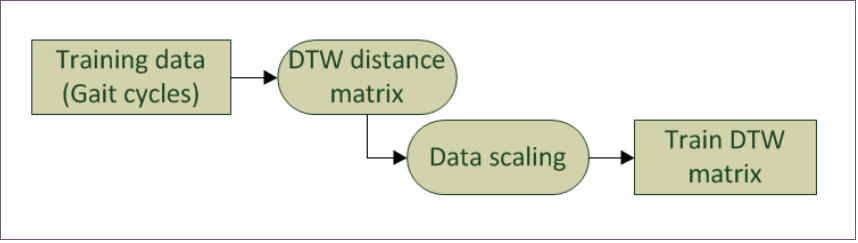
\psfig{file=TrainingData.png,width =3in}
%\caption{Preparing data for SVM}
%\label{fig:TD3}
%\end{figure}

%@@@@@@@@@@@@@@@@@@@@@@@@@@@@@@@@@@@@@@@@@@@@@@@@%	

\subsubsection{Machine Learning Classification}
	The machine learning classification uses the same approaches in \ref{FPP} and \ref{FFE} for preprocessing and gait feature extraction. An additional step is added before gait classification. Once the gait cycles are extracted, they are separated into two groups. 80\% go into a training data set, while 20\% go into a testing data set. The DTW distance matrix is computed using the training data set.

	SVMs are used to classify gait data and are often used for biometric recognition where imposter and genuine data have to be determined. First the SVM finds a \textit{hyperplane}. A hyperplane is a subspace that is one dimension less than its ``ambient space''. For example, there could a 3-dimensional plane represented by 3 axes (X,Y,Z). The hyperplane of the 3-dimensional plane would be the same as a 2-dimensional plane containing 2 axes (X and Y). The SVM will analyze the data, in order to find a hyperplane that linearly separates \begin{math}\mathcal{D} \end{math} dimensional data into two classes. The dimensional data must be linearly separable for the SVM to work. Since the gait data is not linearly separable, a ``kernel induced feature space''~\cite{Muaaz:2013} is introduced in the SVM. A kernel function maps non linearly separable data to a high-dimensional space. Once mapped to a high-dimensional space, the data is linearly separable and, therefore, can be used by the SVM to find a hyperplane. This means that, depending on the kernel function you use, it will produce better classification accuracy. 

There are kernel functions that would require the use of fixed length gait cycles. Since gait cycles are not usually of a fixed-length, a different kernel is used. By using the DTW distance, the problem of fixed-length input feature vectors can be solved as well as more accurate finding of similarity in the data. Two different approaches using SVM and DTW can be used to classify gait cycles: Pre-computed data matrix and Pre-computed kernel.

\subsubsection*{Precomputed Data Matrix}
	Gait cycles are represented by the DTW distance. The DTW distance is the distance between two gait cycles. The benefit of the DTW distance is that gait cycles with different lengths can be compared. A DTW matrix is computed by taking the sample DTW distance and comparing it to all other samples. This matrix is needed as an input for the SVM.	

\subsubsection*{Pre-computed Kernel}
Using \textit{gaussian dynamic time warping} (GDTW) kernel equation~\eqref{eq:KF3} as the kernel matrix also allows for the classification of the gait data. Though this kernel matrix is a symmetric matrix, it is not guaranteed that it has all positive eigenvalues. 
\begin{equation} \label{eq:KF3}
K(x,z)=exp(-\gamma \parallel DTW(x,z) \parallel ^2)
\end{equation}	

	
%\subsubsection{Machine learning based classification}

\subsection{Unfixed Method Gait Classification}
The framework used for classifying gait cycles is a Gaussian Mixture Model-Universal Background Model (GMM-UBM). The algorithm can be split into three primary sections: UBM training, user gait model genertion, runtime inference and adaptation. 

	 The UBM is a large, Universal background GMM that is trained from a large source of data. This means a UBM represents the general walk pattern of humans. The UBM is defined as 
\begin{math} \lambda \end{math} (\begin{math} \omega \end{math},
\begin{math} \upmu \end{math},
\begin{math} \Sigma \end{math}) where
\begin{math} \omega \end{math} represents the mixture weight, \begin{math} \upmu \end{math} represents the mean, and \begin{math} \Sigma \end{math} represents the covariance matrix. In other words, \begin{math} \omega \end{math} is the prior distribution of walking patterns while \begin{math} \upmu \end{math} and \begin{math} \Sigma \end{math} are different walking patterns given by the population in different conditions. For efficiency the \textit{covariance matrix} is used. A covariance matrix ``generalizes the notion of variance to multiple dimensions.''\cite{Lu:2014} To avoid overfitting the training data, a standard expectation maximization (EM) algorithm is applied. The EM trains the UBM models. For example, if given a collection of training vectors, the EM estimates the parameters most likely to occur. The EM algorithm does this through iteration. Each time the algorithm iterates it refines the GMM parameters, increasing the likelihood of the estimated model for the given feature vectors. 
%maybe provide an example?????

	The individual user's gait model is a GMM, but instead of using EM training, a Bayesian adaptation is used. This relates the odds of one event to the odds of another. The Bayesian adaptation is both used for performance as well as for its ability to learn from the data. The Maximum-a-Posteriori (MAP) is the adaptation used. The MAP adaptation adjusts the Gaussian components and mixture weight to personalize the UBM model. MAP is also used at runtime to learn new gait patterns from the user. MAP does this by recording false negatives, indicated by the user, by providing an alternate form of authentication. 

	
%	It is during runtime that the extracted features are compared against the user gait model and the UBM creating a score. High scores result from the user model being higher than the UBM model and visa versa for low scores. These scores are computed as \begin{equation}
%	\Updelta = log(p(X|\lambda_{user})) - log(p(X|\lambda_{ubm}))
%	\end{equation}
%In this equation \begin{math} \Updelta \end{math} is equal to the user's score, X is the feature vector, and \begin{math} \lambda \end{math} represents the type of model the feature vector is being compared against.%

%7777777777777@@@@@@@@@@@@@@@@@@@@@@@@@@@@@@@@@@@@@@@@@@@@@@@@%
\begin{figure}
\centering
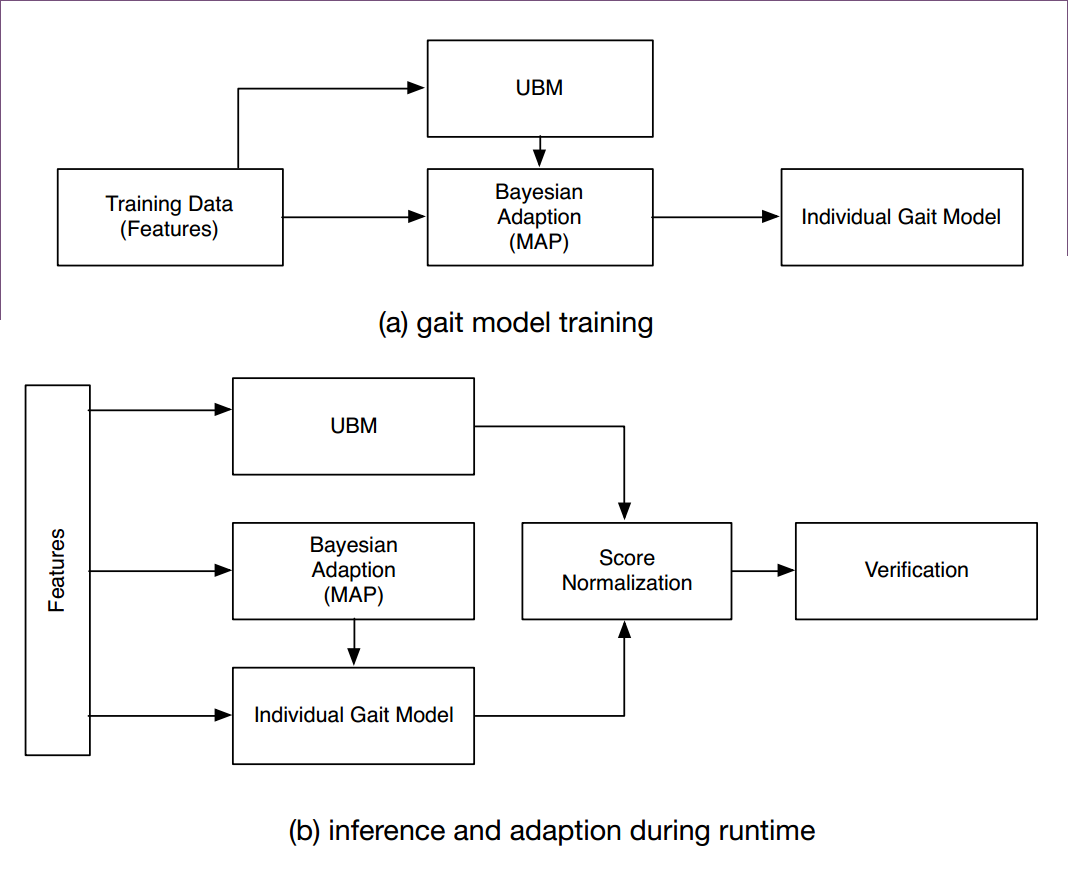
\psfig{file=FESP.png,width =3in}
\caption{Algorithm work-flow for (a) generate user gait model by MAP adaptation (b) runtime inference and Individual model adaptation}
\label{fig:TD2}
\end{figure}
%@@@@@@@@@@@@@@@@@@@@@@@@@@@@@@@@@@@@@@@@@@@@@@@@%

%\section{Experiment Results}
%\subsubsection{Paper 1(title place holder)}
%\subsubsection{Paper 2(title place holder)}


%88888888888@@@@@@@@@@@@@@@@@@@@@@@@@@@@@@@@@@@@@@@@@@@@@@@@%
%\begin{figure}
%\centering
%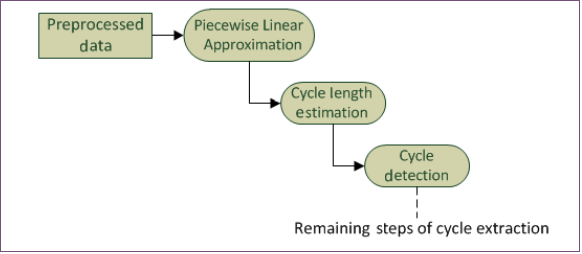
\psfig{file=PreprocessedData.png,width =3in}
%\caption{Gait cycle extraction steps with Piecewise Linear Approximation (PLA)}
%\label{fig:AddedStep}
%\end{figure}
%@@@@@@@@@@@@@@@@@@@@@@@@@@@@@@@@@@@@@@@@@@@@@@@@%

	
%777777777777777777777777777777777777777777777777777777777777777777777777777777777777
\section{Conclusion}
	
	
	Two experiments where conducted by the research group who implemented the fixed method approach. One experiment used PLAs for gait classification, while the other used SVMs for gait classification. Both experiments show benefits and drawbacks to using either technique. Using PLAs will speed-up the processing time to approximately 2-3 minutes. Though faster, using PLAs will increase EERs from 16.26\% (without PLAs) to 22.49\% (with PLAs). Unlike the first experiment, the second experiment has the benefit of being able to handle gait cycles of different lengths. Two approaches using SVMs were developed: pre-computed data matrices, and pre-computed kernel. Pre-computed data matrices were used to train and test SVMs, but relied on having trained models and training data. The pre-computed kernel approach did not rely on having training models or training data. Using SVMs, a TER of 36.82\% was achieved. 
	
%	 Though only gait cycles of the same length were used, DTW allows for future work with gait cycles of variable lengths. Future work will involve recording at higher sampling rate (varying frequencies) as well as placing the phone in more realistic positions on the body.%
		
		The research group, who implemented the unfixed method approach, conducted three experiments using: a data set used for training walking a walking detector and UBM, a data set used for evaluating supervised training of gait models, and a data set used for evaluating unsupervised training. The main focused for each experiment was training the data. For each experiment, using larger training data sets, up to 10\% of the data, increased the accuracy. The best EER was 14\% and the average processing time was approximately 0.0279 seconds. By using the unfixed approach, this research group was able to have a better EER by 2.26\% and a large improvement in processing time going from minutes, to less than a second.

	Two forms of gait recognition have been compared using very similar strategies to create an unobtrusive security process for mobile phones using stock Android phones. Using Android phones allows for each method to use similar, if not the same accelerometers, giving both methods access to the same data. The difference between these two methods are: placement of the mobile device, their different implementations of the strategies to which their algorithms were built, and their context of use. Though the fixed method was implemented using a controlled setting and the unfixed method was geared to more real-life implementations, they both show promise for future work. 
\section{Acknowledgments}
	I would like to thank Kristin Lamberty and Elena Mach\-kasova for their advice and feedback as well as Melissa Helgeson for additional feedback and proofreading. 
% The following two commands are all you need to
% produce the bibliography for the citations in your paper.
\bibliographystyle{abbrv}
% annotated_bibliography.bib is the name of the BibTex file containing 
% all the bibliography entries for this example. Note that you *don't* include the .bib ending
% in the \bibliography command.



\bibliography{paper}  

% You must have a ".bib" file and remember to run:
%     pdflatex bibtex pdflatex pdflatex
% in order to see all the citation references correctly.

%
%\begin{displaymath}
%K : X \times X \rightarrow \mathbb{R}, \forall \{x,z\} \in X
%\label{eq:KF1} 
%\end{displaymath}
%
%\begin{displaymath}
%K(x,z)=< \phi (x).\phi(z) > 
%\label{eq:KF2}
%\end{displaymath}

\end{document}



